%\section {Pianificazione}
\section {Pianificazione}
\subsection {Introduzione}
	\subsubsection{Scelta modello di sviluppo}
	Il modello di \glo{Ciclo di vita}{ciclo di vita} scelto per il prodotto è il modello incrementale, che suddivide lo
	svolgimento del progetto in varie \glo{Fase}{fasi} significative. Questo modello permette inoltre di:
	\begin{itemize}
		\item valorizzare i requisiti principali nelle prime \glo{Fase}{fasi} di sviluppo, dedicandosi successivamente
		ai requisiti opzionali;
		\item minimizzare i rischi di ritardo rispetto ai tempi stabiliti in quanto, le \glo{Fase}{fasi}, hanno durata
		breve e sono precedentemente pianificate;
		\item semplificare l’attività di verifica.
	\end{itemize}
	\subsubsection {Scelta consegna RP}
	Il \glo{Gruppo}{gruppo} ha scelto di consegnare alla \revprog{} i risultati della progettazione di alto livello al fine di identificare tempestivamente errori concettuali, riducendone quindi il costo di correzione.
	%\subsubsection{Dipendenze fra le attività}
	\subsubsection{Fasi e milestones}
	Si è deciso di fissare una \glo{Milestone}{milestone} in corrispondenza di ogni scadenza stabilita nella sezione \ref{subsec:scadenze}. Dopo aver identificato le attività da svolgere, i vincoli e rischi (vedi sezione \ref{sec:analisirischi}) a cui il progetto è sottoposto, il \glo{Gruppo}{gruppo} ha deciso di suddividere il tempo utile in \glo{Fase}{fasi}. Ogni \glo{Fase}{fase} termina 4 giorni prima di una \glo{Milestone}{milestone}; il tempo in eccesso potrà essere usato in caso di ritardi nel completamento delle attività.\\

	\begin{table}[ht]
		\footnotesize\setlength{\tabcolsep}{6pt}
		\begin{center}
			\begin{tabular}{lllll}
				\toprule
				ID fase & Nome fase                                             & Inizio                        & Fine                          & Relativa milestone                            \\
				\midrule
				An      & Analisi                                               & \frmdata{01}{12}{2016}  & \frmdata{07}{01}{2017}  & RR - \frmdata{11}{01}{2017}                  \\
				\midrule
				Pl      & Progettazione logica                                  & \frmdata{12}{01}{2017}  & \frmdata{02}{03}{2017}  & RP - \frmdata{06}{03}{2017}                  \\
				\midrule
				PdROb   & Prog. dettaglio e codifica dei Requisiti Obbligatori  & \frmdata{07}{03}{2017}  & \frmdata{22}{03}{2017} & \multirow{3}{*}{RQ - \frmdata{11}{04}{2017}} \\
				PdRD    & Prog. dettaglio e codifica dei Requisiti Desiderabili & \frmdata{23}{03}{2017} & \frmdata{02}{04}{2017}  &                                               \\
				PdROp   & Prog. dettaglio e codifica dei Requisiti Opzionali    & \frmdata{03}{04}{2017}  & \frmdata{07}{04}{2017}  &                                               \\
				\midrule
				Va      & Validazione                                           & \frmdata{12}{04}{2017} & \frmdata{04}{05}{2017}  & RA - \frmdata{08}{05}{2017}  \\
				\bottomrule
			\end{tabular}
		\end{center}
		\caption{Fasi e milestones}
		\label{tab:fasi}
	\end{table}\mbox{}\\

\subsection{Assegnazione delle attività alle fasi}
	I processi e le attività assegnate ad ogni \glo{Fase}{fase} nelle seguenti sezioni del documento sono state descritte nelle \ndpv:

	\subsubsection {Analisi}
		\textbf{Periodo}: da \frmdata{01}{12}{2016} a \frmdata{07}{01}{2017} (38 giorni) \\
		Durante questa \glo{Fase}{fase} vengono valutati i vari capitolati proposti e dopo aver scelto un determinato \glo{Capitolato}{capitolato}, vengono gestite principalmente la contrattazione e la raccolta di requisiti.
		\paragraph{Processi e attività coinvolte}
			\begin{table}[H]
				\centering
				\begin{tabular}{ll}
					\toprule
					\textbf{Processo}                           & \textbf{Attività}              \\
					\midrule
					\multirow{2}{*}{\textbf{Fornitura}}         & Studio di Fattibilità          \\
					& Contrattazione                 \\
					\midrule
					\textbf{Sviluppo}          & Analisi dei requisiti          \\
					\midrule
					\textbf{Documentazione}            & Produzione dei documenti       \\
					\midrule
					\textbf{Verifica}                  & Verifica                       \\
					\midrule
					\textbf{Gestione processi} 					& Gestione processi              \\
					\midrule
					\textbf{Gestione infrastrutture}				& Gestione infrastrutture        \\
					\midrule
					\textbf{Apprendimento} 						& Apprendimento                 \\
					\bottomrule
				\end{tabular}
				\caption{Processi e relative attività}
				\label{An-ProcessiAttività}
			\end{table}
		\paragraph{Diagramma di Gantt}
		\begin{figure}[H]
			\centering
			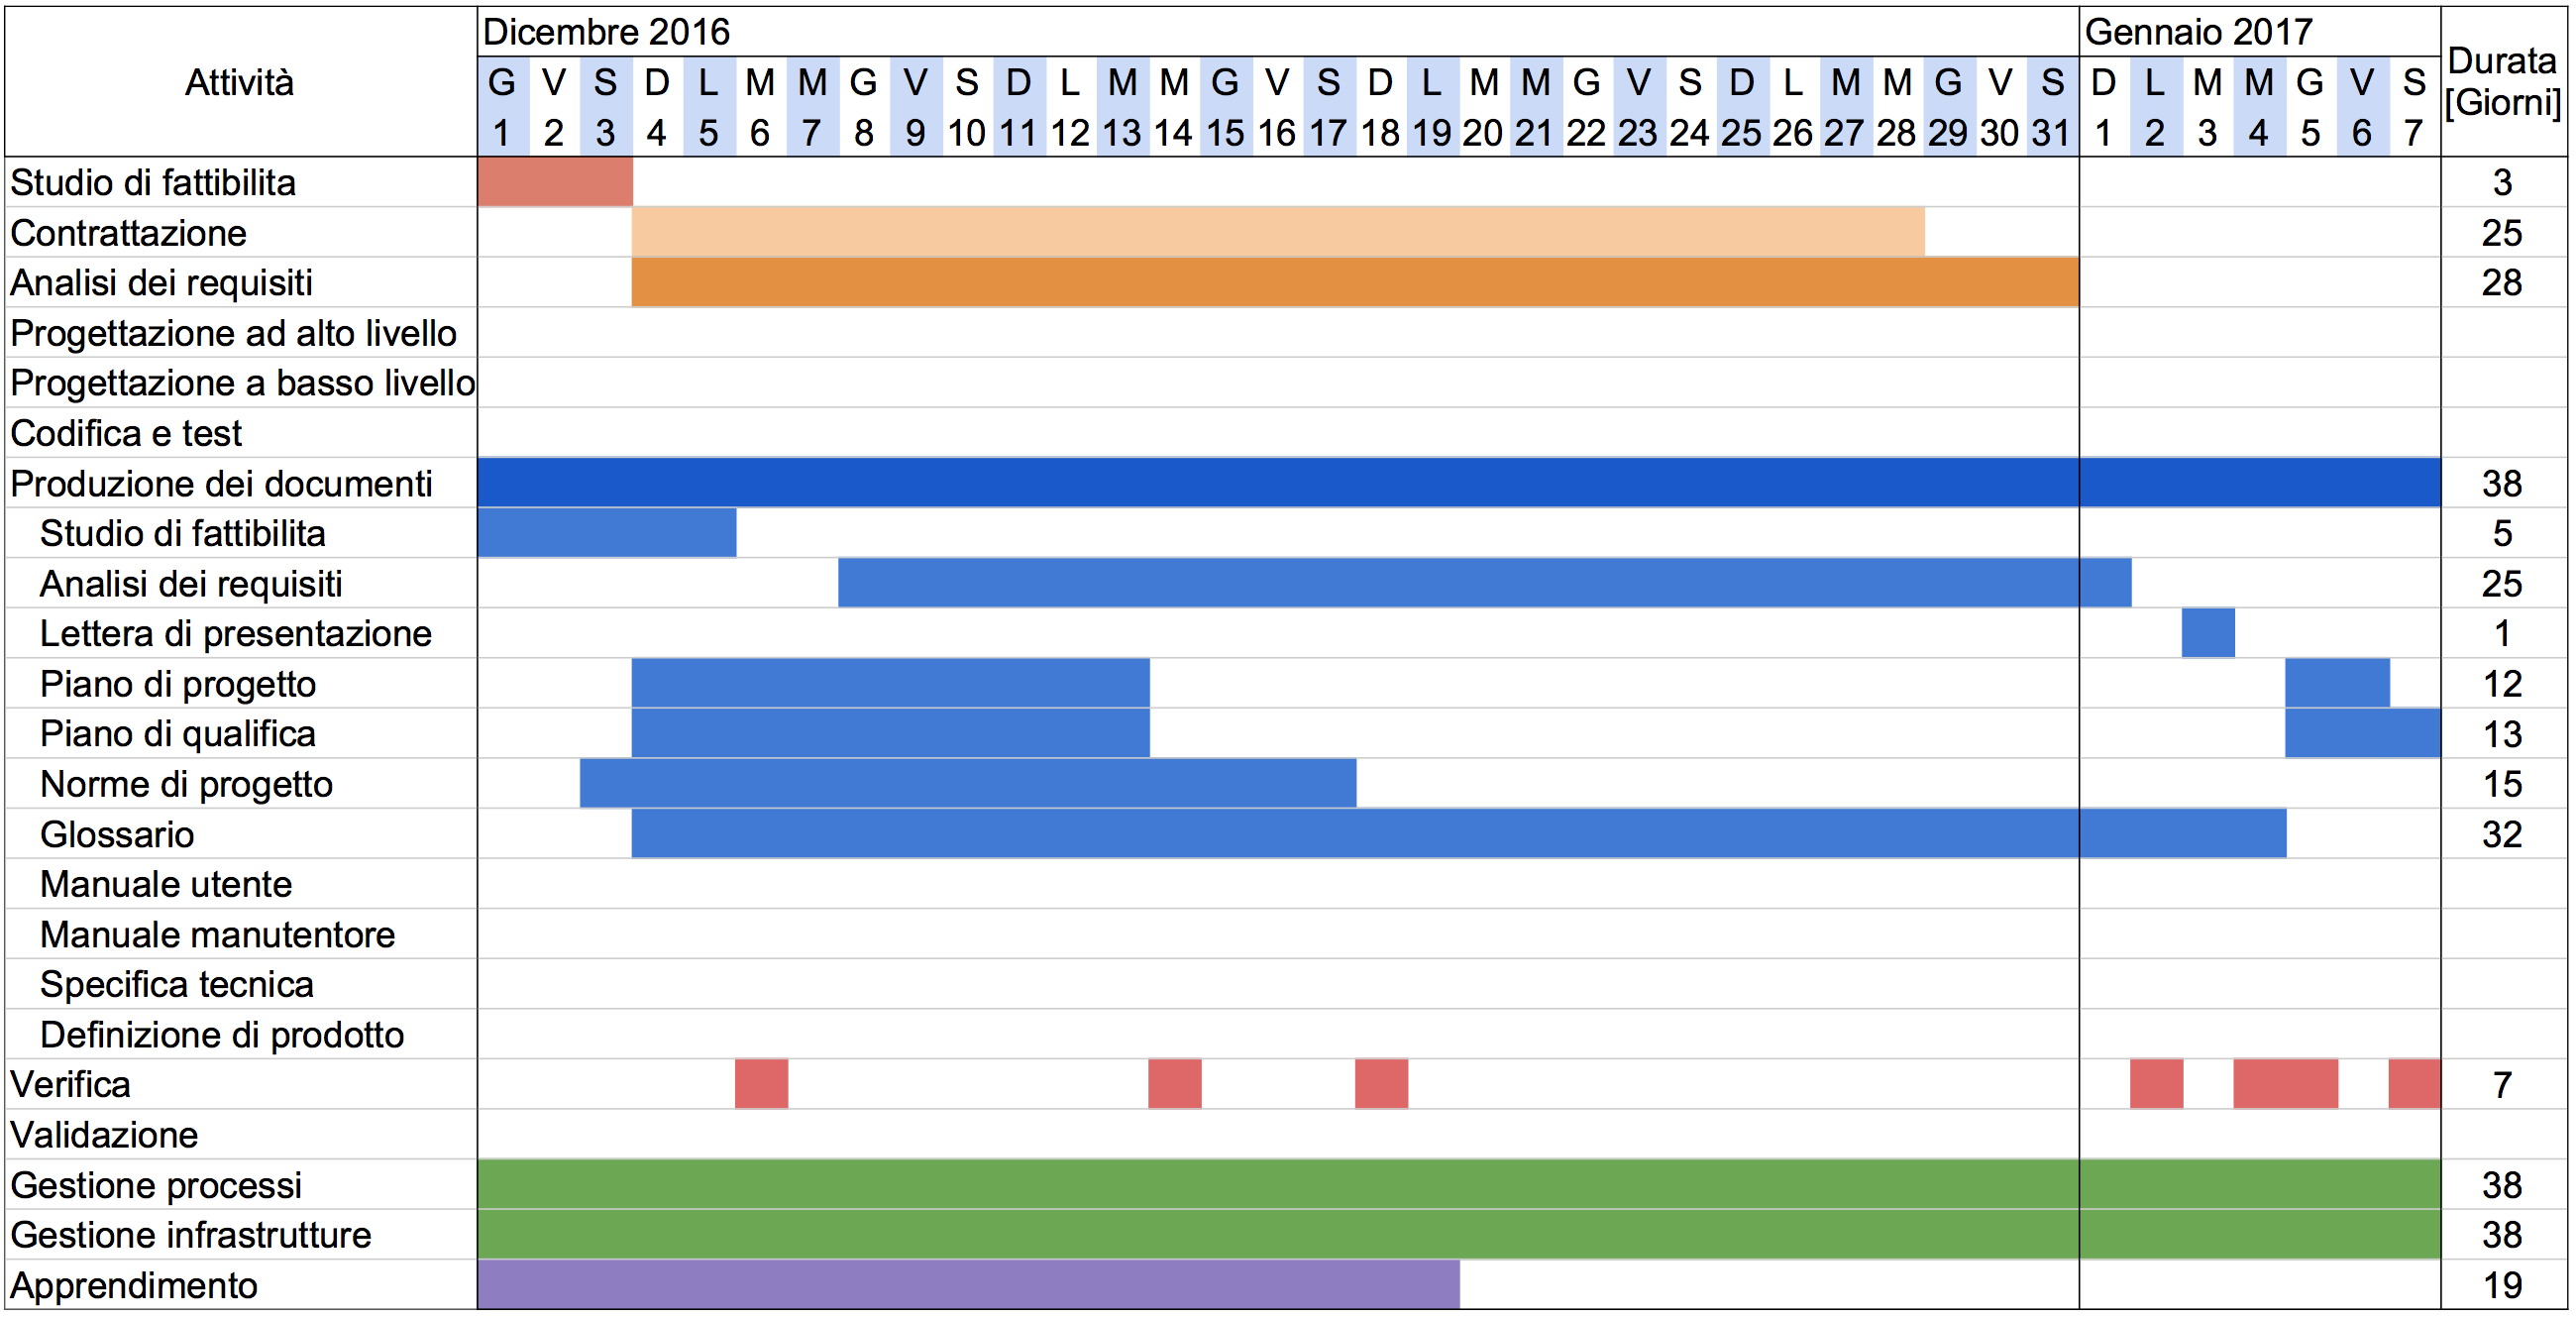
\includegraphics[width=\textwidth]{img/Gantt/f1c.png}
			\caption{Diagramma di Gantt - Fase di analisi}
		\end{figure}
	\subsubsection {Progettazione logica}
		\textbf{Periodo}: da \frmdata{12}{01}{2017} a \frmdata{02}{03}{2017} (50 giorni) \\
		Durante questa \glo{Fase}{fase} continua la raccolta di requisiti e comincia la progettazione ad alto livello del prodotto.
		\paragraph{Processi e attività coinvolte}
			\begin{table}[H]
				\centering
				\begin{tabular}{ll}
					\toprule
					\textbf{Processo}                           & \textbf{Attività}              \\
					\midrule
					\multirow{2}{*}{\textbf{Sviluppo}}          & Analisi dei requisiti          \\
					& Progettazione ad alto livello  \\
					\midrule
					\textbf{Documentazione}            & Produzione dei documenti       \\
					\midrule
					\textbf{Verifica}                  & Verifica                       \\
					\midrule
					\textbf{Gestione processi} 					& Gestione processi              \\
					\midrule
					\textbf{Gestione infrastrutture}				& Gestione infrastrutture        \\
					\midrule
					\textbf{Apprendimento} 						& Apprendimento                 \\
					\bottomrule
				\end{tabular}
				\caption{Processi e relative attività}
				\label{Pl-ProcessiAttività}
			\end{table}
		\paragraph{Diagramma di Gantt}
		\begin{figure}[H]
			\centering
			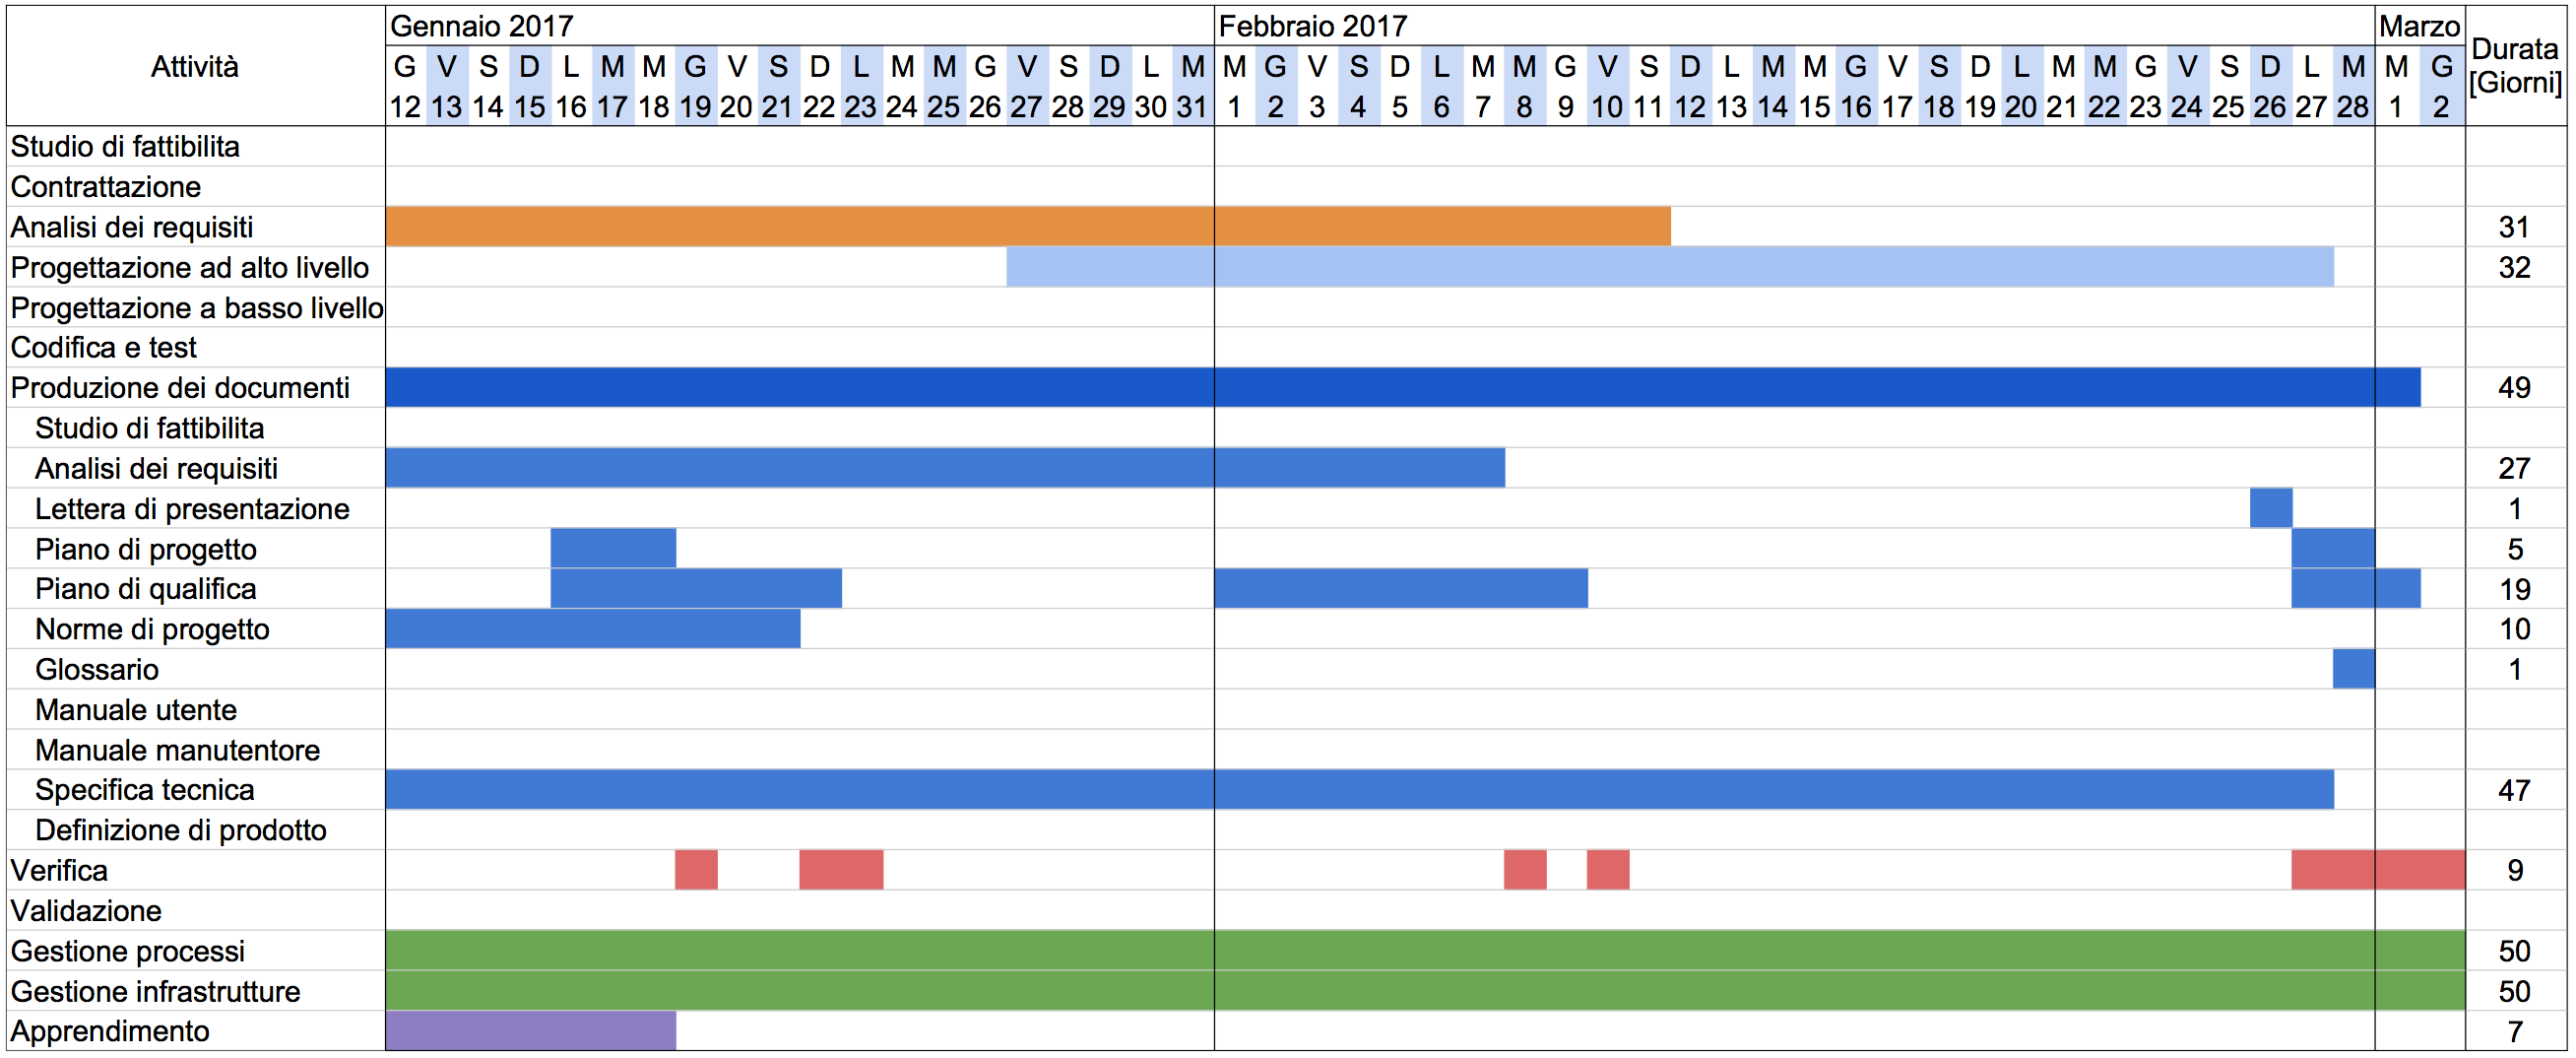
\includegraphics[width=\textwidth]{img/Gantt/f2c.png}
			\caption{Diagramma di Gantt - Fase di progettazione logica}
		\end{figure}
	\subsubsection {Progettazione di dettaglio e codifica requisiti obbligatori}
		\textbf{Periodo}: da \frmdata{07}{03}{2017} a \frmdata{22}{03}{2017} (16 giorni)\\
		Durante questa \glo{Fase}{fase} vengono presi in considerazione i requisiti obbligatori e vengono codificati dopo la progettazione a basso livello.
		\paragraph{Processi e attività coinvolte}
			\begin{table}[H]
				\centering
				\begin{tabular}{ll}
					\toprule
					\textbf{Processo}                           & \textbf{Attività}              \\
					\midrule
					\multirow{2}{*}{\textbf{Sviluppo}}          & Progettazione ad basso livello \\
					& Codifica e test \\
					\midrule
					\textbf{Documentazione}            & Produzione dei documenti       \\
					\midrule
					\textbf{Verifica}                  & Verifica                       \\
					\midrule
					\textbf{Gestione processi} 					& Gestione processi              \\
					\midrule
					\textbf{Gestione infrastrutture}				& Gestione infrastrutture        \\
					\midrule
					\textbf{Apprendimento} 						& Apprendimento                 \\
					\bottomrule
				\end{tabular}
				\caption{Processi e relative attività}
				\label{Pdrob-ProcessiAttività}
			\end{table}
		\paragraph{Diagramma di Gantt}
		\begin{figure}[H]
			\centering
			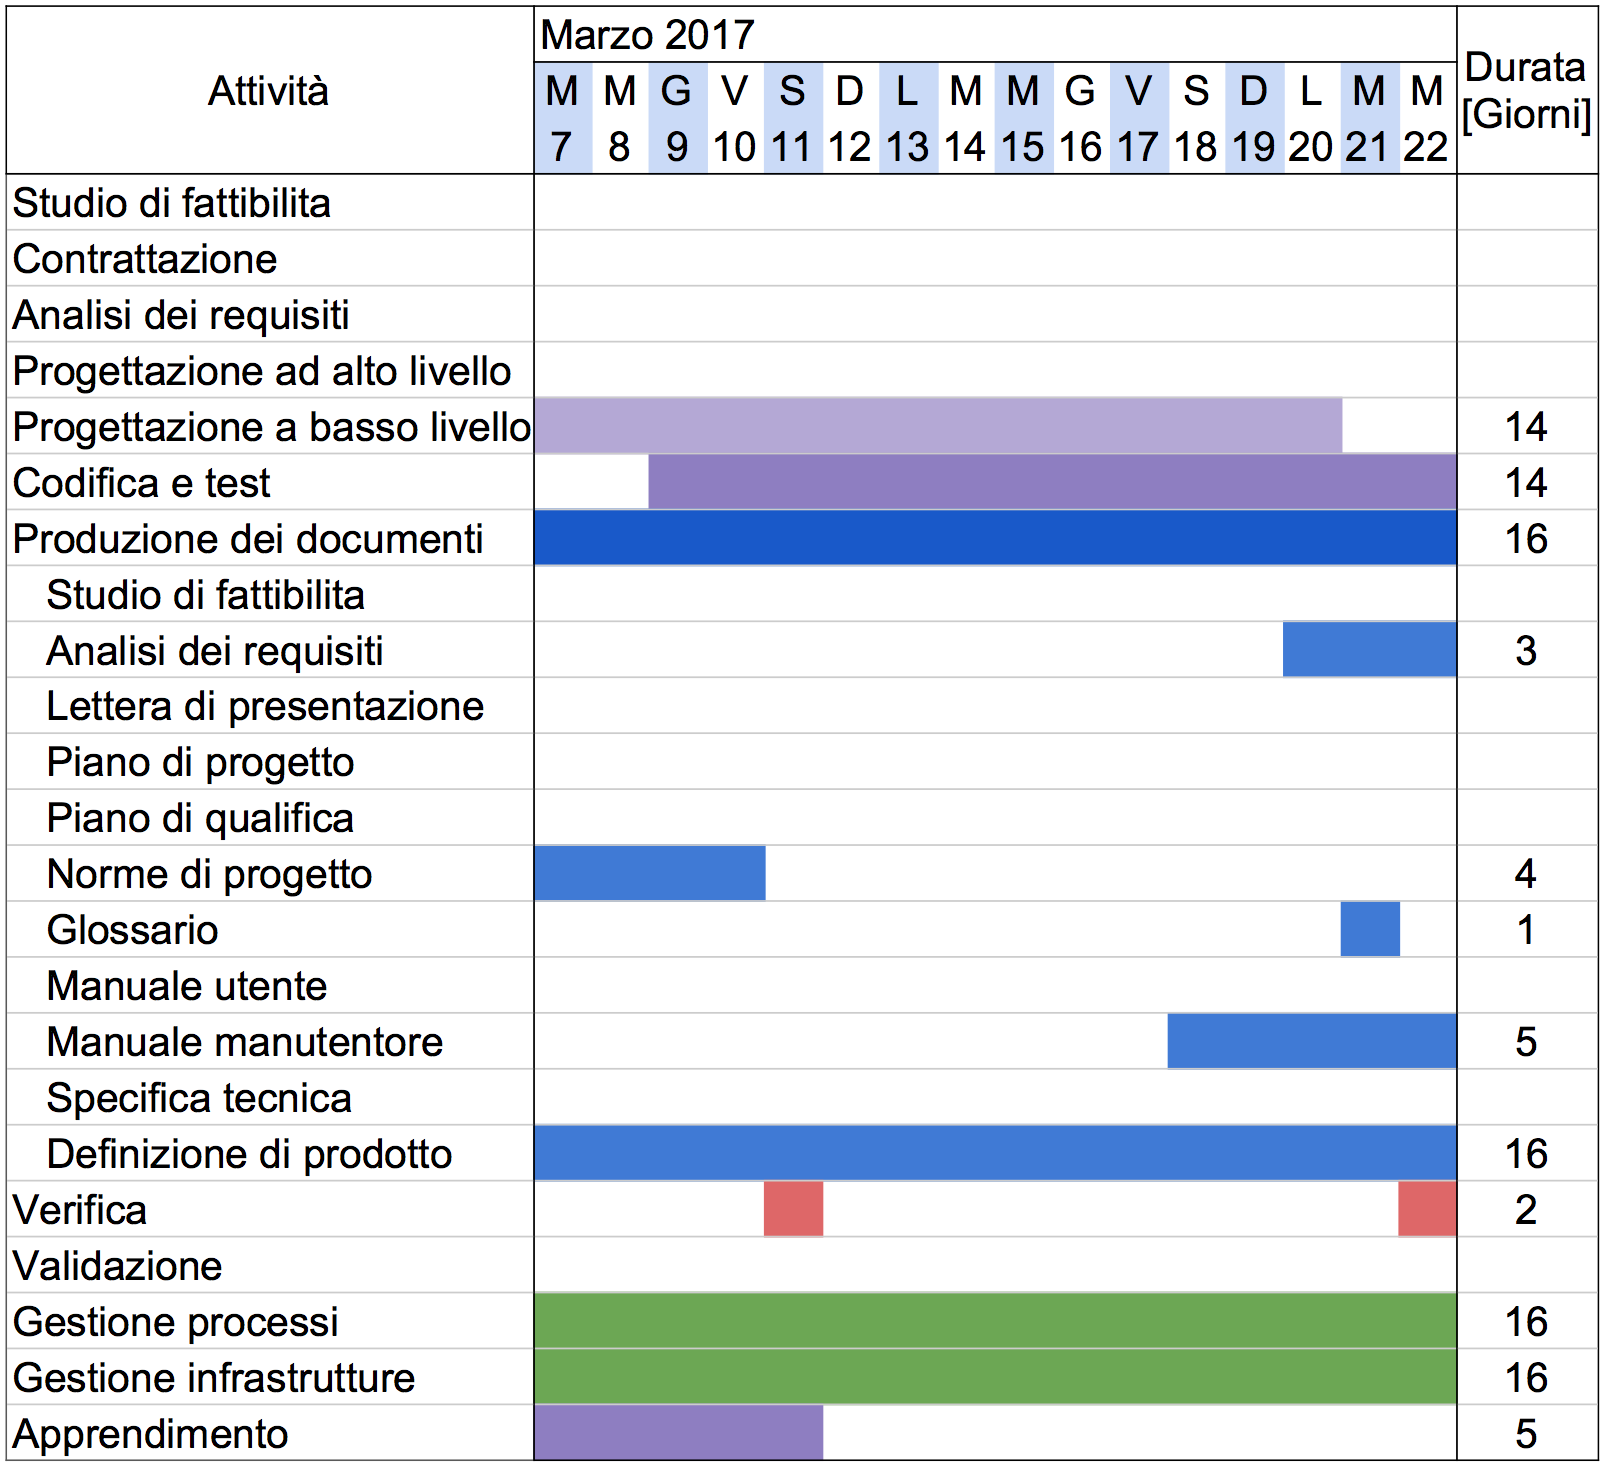
\includegraphics[height=0.45\textheight]{img/Gantt/f3c.png}
			\caption{Diagramma di Gantt - Fase di progettazione di dettaglio e codifica requisiti obbligatori}
		\end{figure}
	\subsubsection {Progettazione di dettaglio e codifica requisiti desiderabili}
		\paragraph{Processi e attività coinvolte}
			\textbf{Periodo}: da \frmdata{23}{03}{2017} a \frmdata{02}{04}{2017} (11 giorni) \\
			Durante questa \glo{Fase}{fase} vengono presi in considerazione i requisiti desiderabili e vengono codificati dopo la progettazione a basso livello.
			\begin{table}[H]
				\centering
				\begin{tabular}{ll}
					\toprule
					\textbf{Processo}                           & \textbf{Attività}              \\
					\midrule
					\multirow{2}{*}{\textbf{Sviluppo}}          & Progettazione ad basso livello \\
					& Codifica e test \\
					\midrule
					\textbf{Documentazione}            & Produzione dei documenti       \\
					\midrule
					\textbf{Verifica}                  & Verifica                       \\
					\midrule
					\textbf{Gestione processi} 					& Gestione processi              \\
					\midrule
					\textbf{Gestione infrastrutture}				& Gestione infrastrutture        \\
					\midrule
					\textbf{Apprendimento} 						& Apprendimento                 \\
					\bottomrule
				\end{tabular}
				\caption{Processi e relative attività}
				\label{Pdrd-ProcessiAttività}
			\end{table}
		\paragraph{Diagramma di Gantt}
		\begin{figure}[H]
			\centering
			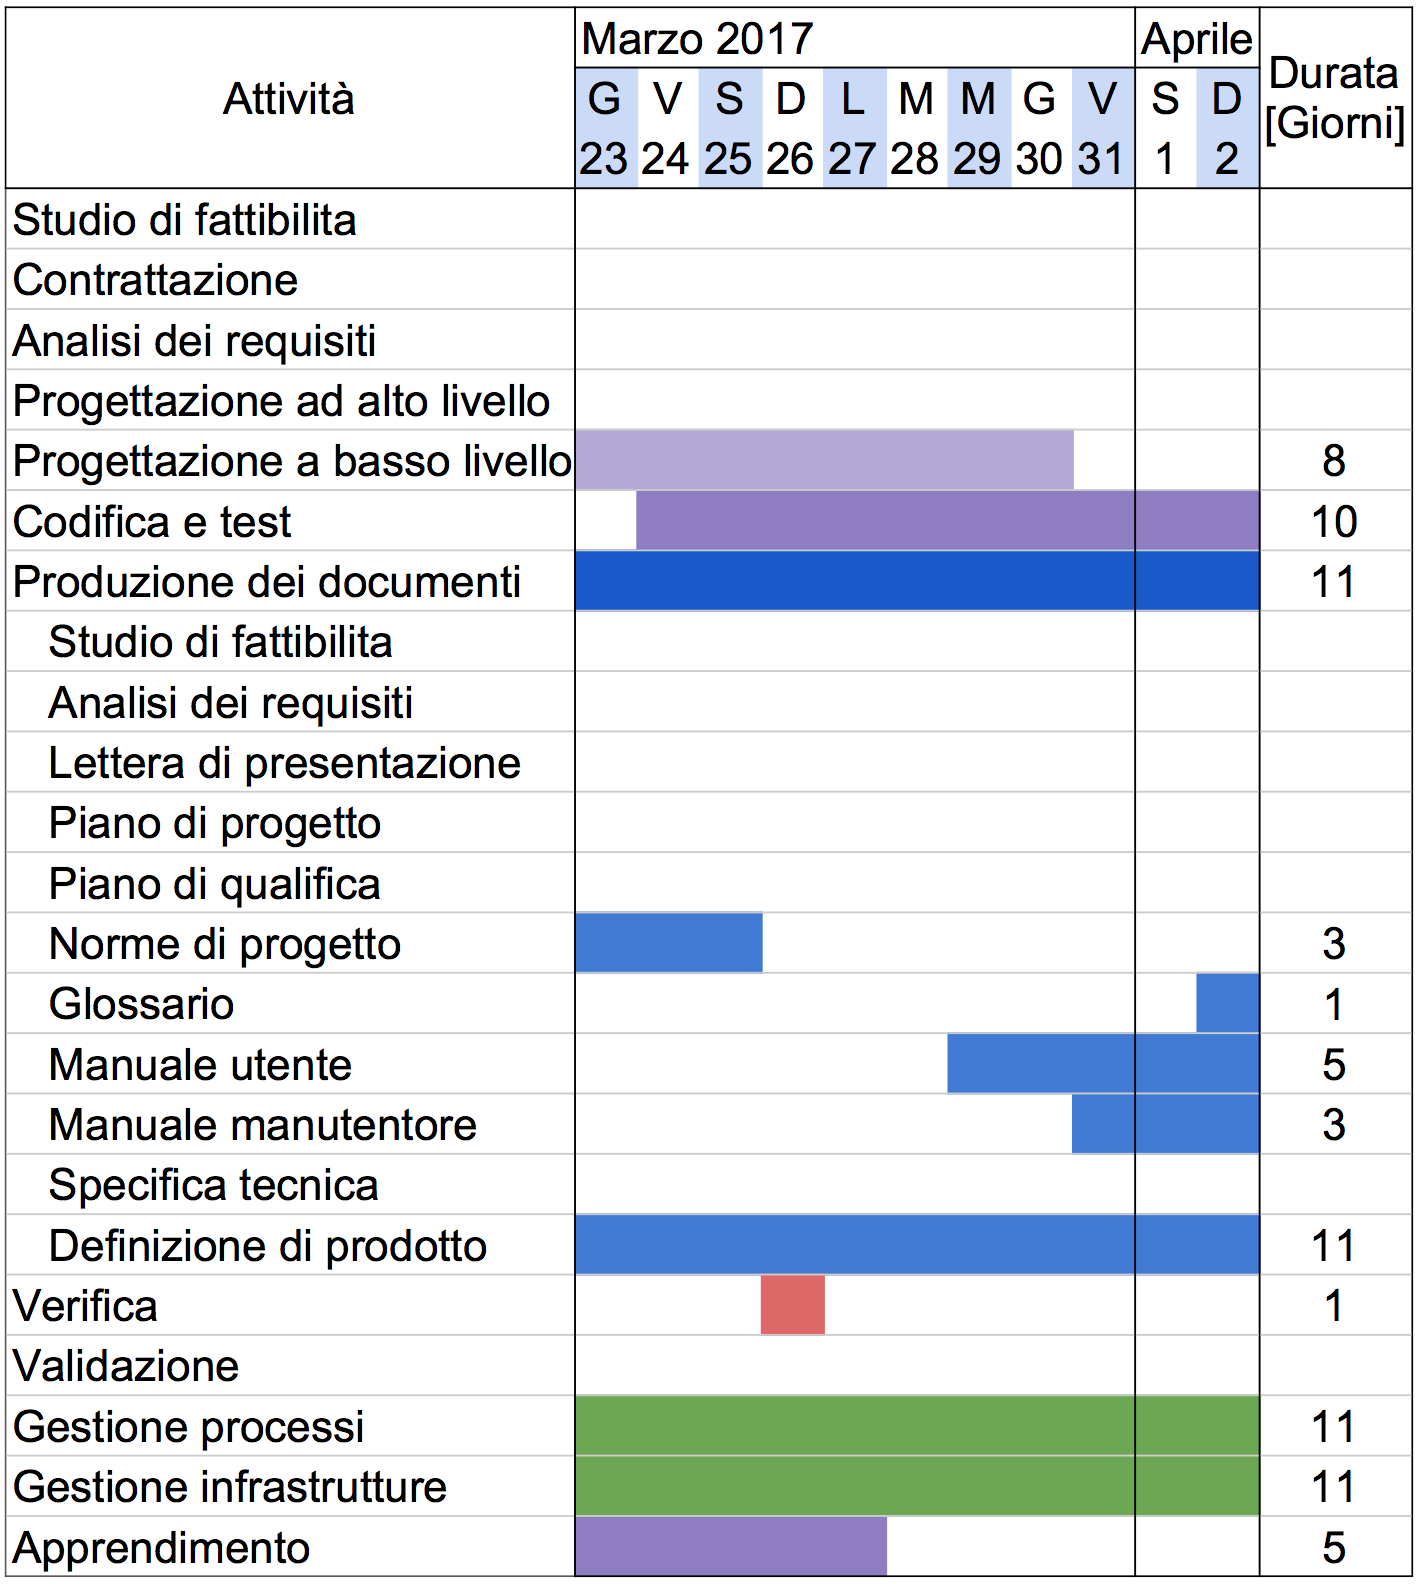
\includegraphics[height=0.45\textheight]{img/Gantt/f4c.png}
			\caption{Diagramma di Gantt - Fase di progettazione di dettaglio e codifica requisiti desiderabili}
		\end{figure}
	\subsubsection {Progettazione di dettaglio e codifica requisiti opzionali}
		\paragraph{Processi e attività coinvolte}
			\textbf{Periodo}: da \frmdata{03}{04}{2017} a \frmdata{07}{04}{2017} (5 giorni) \\
			Durante questa \glo{Fase}{fase} vengono presi in considerazione i requisiti opzionali e vengono codificati dopo la progettazione a basso livello.
			\begin{table}[H]
				\centering
				\begin{tabular}{ll}
					\toprule
					\textbf{Processo}                           & \textbf{Attività}              \\
					\midrule
					\multirow{2}{*}{\textbf{Sviluppo}}          & Progettazione ad basso livello \\
					& Codifica e test \\
					\midrule
					\textbf{Documentazione}            & Produzione dei documenti       \\
					\midrule
					\textbf{Verifica}                  & Verifica                       \\
					\midrule
					\textbf{Gestione processi} 					& Gestione processi              \\
					\midrule
					\textbf{Gestione infrastrutture}				& Gestione infrastrutture        \\
					\midrule
					\textbf{Apprendimento} 						& Apprendimento                 \\
					\bottomrule
				\end{tabular}
				\caption{Processi e relative attività}
				\label{Pdrop-ProcessiAttività}
			\end{table}
		\paragraph{Diagramma di Gantt}
		\begin{figure}[H]
			\centering
			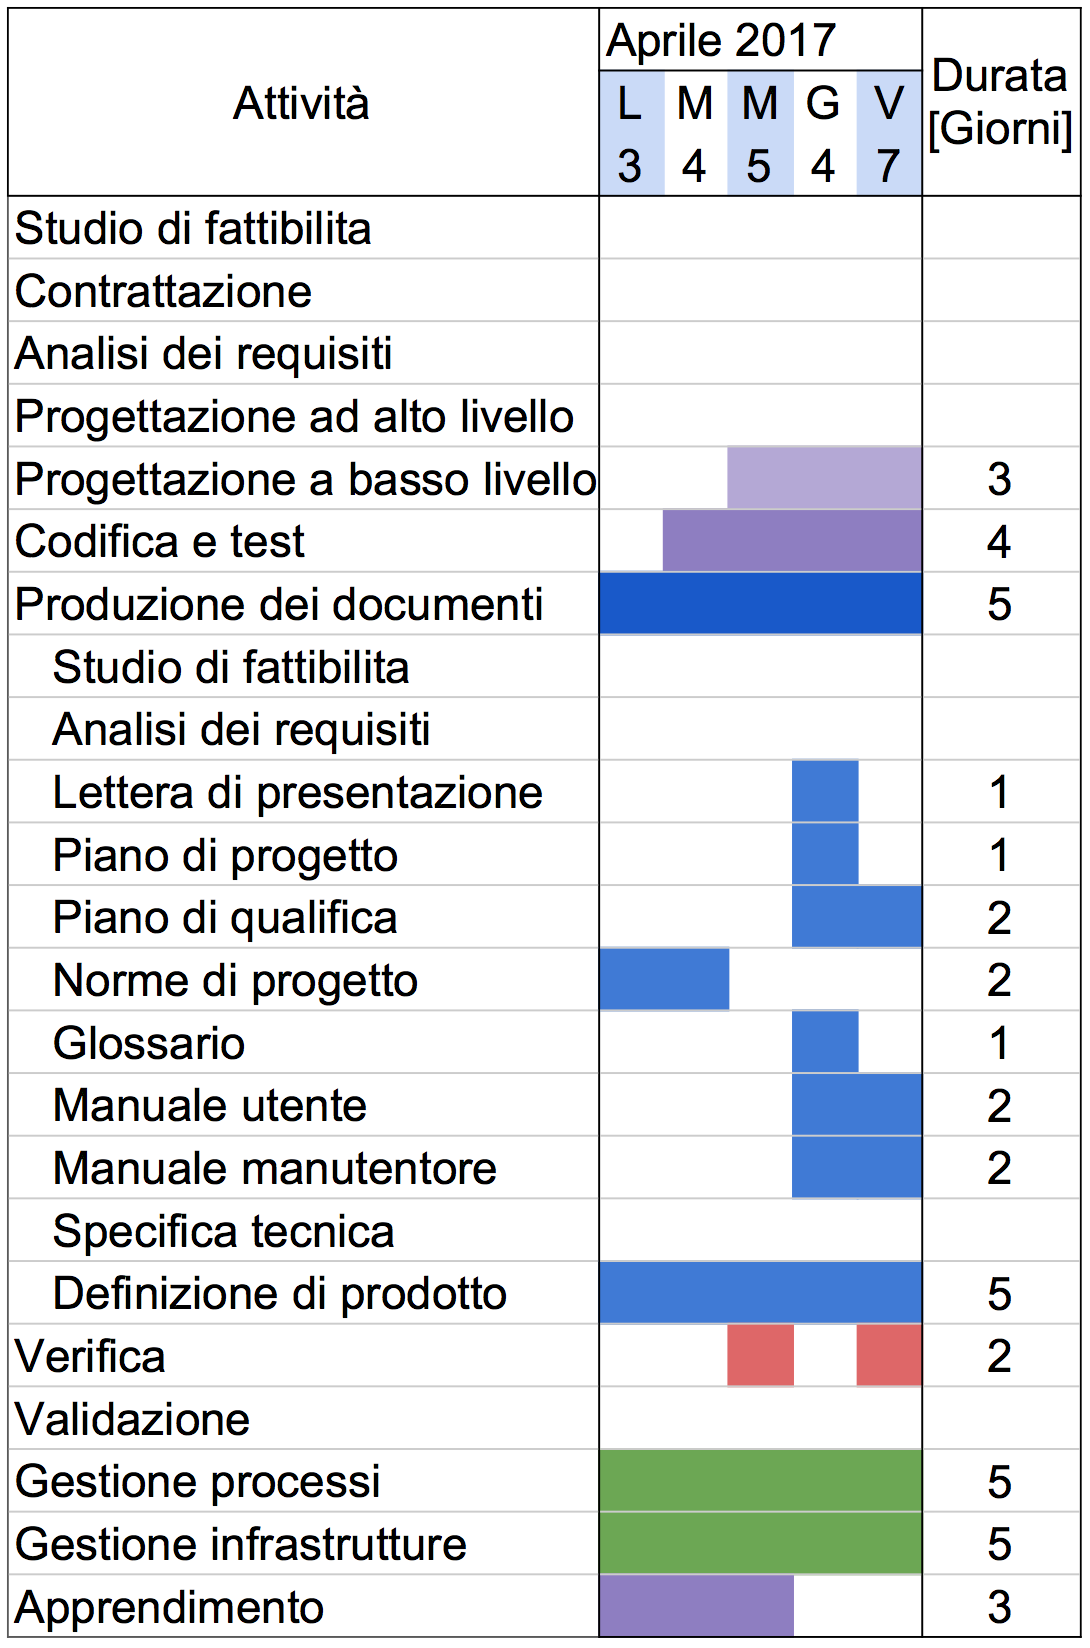
\includegraphics[height=0.45\textheight]{img/Gantt/f5c.png}
			\caption{Diagramma di Gantt - Fase di progettazione di dettaglio e codifica requisiti opzionali}
		\end{figure}
	\subsubsection {Validazione}
		\textbf{Periodo}: da \frmdata{12}{04}{2017} a \frmdata{04}{05}{2017} (23 giorni) \\
		Durante questa \glo{Fase}{fase} vengono validate le varie componenti del prodotto software tramite il controllo dei requisiti e vengono validati i documenti secondo i criteri definiti nelle \glo{Fase}{fasi} precedenti.
		\paragraph{Processi e attività coinvolte}
			\begin{table}[H]
				\centering
				\begin{tabular}{ll}
					\toprule
					\textbf{Processo}                           & \textbf{Attività}              \\
					\midrule
					\textbf{Documentazione}            & Produzione dei documenti       \\
					\midrule
					\textbf{Verifica}                  & Verifica                       \\
					\midrule
					\textbf{Validazione}               & Validazione                    \\
					\midrule
					\textbf{Gestione processi} 					& Gestione processi              \\
					\midrule
					\textbf{Gestione infrastrutture}				& Gestione infrastrutture        \\
					\bottomrule
				\end{tabular}
				\caption{Processi e relative attività}
				\label{Va-ProcessiAttività}
			\end{table}
		\paragraph{Diagramma di Gantt}
		\begin{figure}[H]
			\centering
			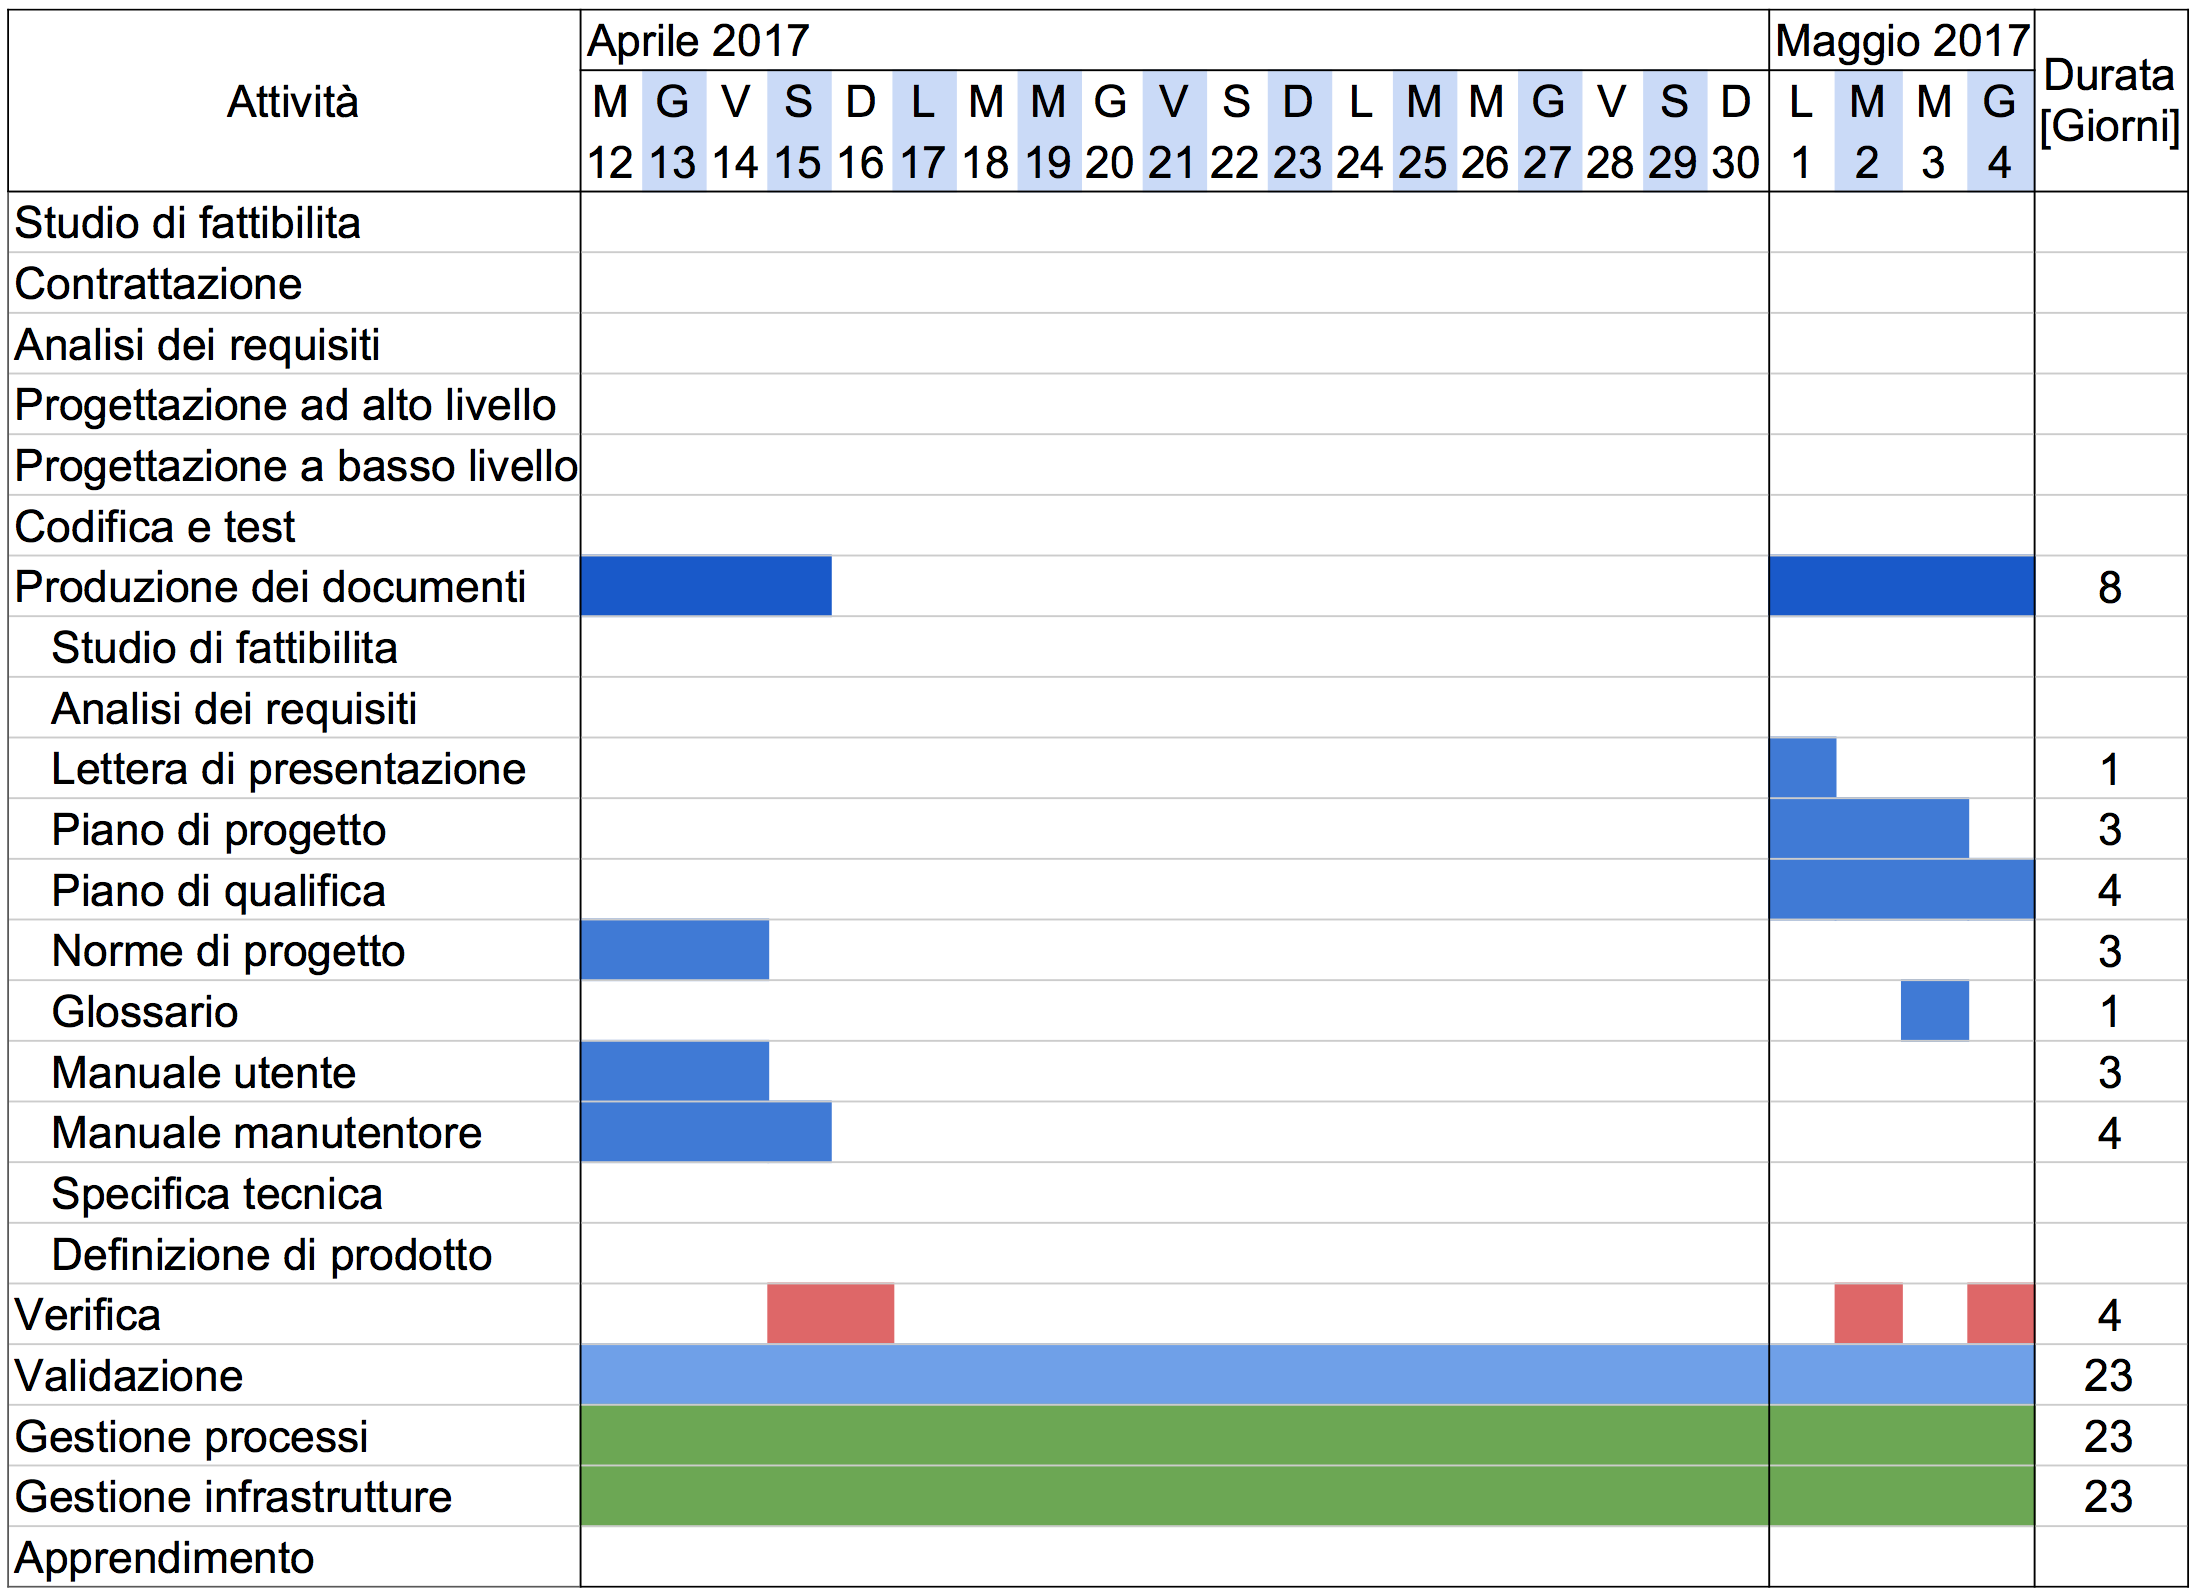
\includegraphics[width=\textwidth]{img/Gantt/f6c.png}
			\caption{Diagramma di Gantt - Fase di validazione}
		\end{figure}
